\chapter{Design\label{chap:design}}
In this chapter, I will talk in depth the elements that I created during this project and how they inter-connect. You can expect a design charts showcasing high-level overview, alongside dividing it onto smaller subsections - each independent and capable of running on its own. I will also provide explanation on novel approaches such as verifying the authenticity of the connecting clients, data model stored on blockchain or how the connection is secured from man-in-the-middle attacks through TLS encryption.

\section{Architecture}
This section includes the diagram of them system and two sample workflows demonstrating how packets are flowing through the framework.
\subsection{Overview}
\begin{figure}[h]
    \centering
    \makebox[\textwidth][c]{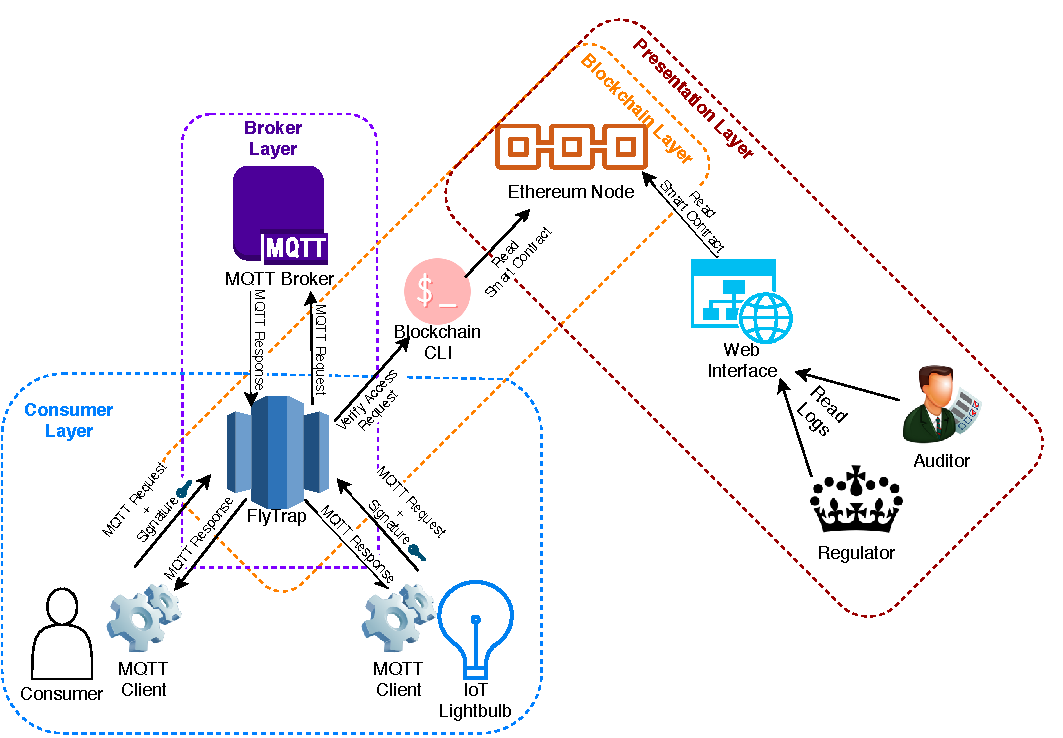
\includegraphics[width=1.2\textwidth]{flytrap}}
    \caption{FlyTrap high-level architecture overview}
    \label{fig:flytrap}
\end{figure}
Figure \ref{fig:flytrap} presents an overview of the system, decomposing it onto four layers, each responsible for different part of the framework. It also demonstrates how those layers are coupled and the direction of data flowing between them.

To overview, we can distinguish four layers:
\begin{description}
    \item[Consumer Layer] - layer responsible for interacting with end-devices. To them, FlyTrap should be indistinguishable from normal MQTT broker and thus accepts/responds with MQTT v5.0 compliant TCP/TLS packets. In order to compute the signature and attach it to 
    \item[Consumer Layer] - layer where FlyTrap acts like a client for MQTT Broker. Similar to Consumer Layer, all packets sent by FlyTrap need to be compliant with MQTT standard in order to receive valid responses from the broker. In this situation, used MQTT broker is not relevant - as long as it implements the standard.
    \item[Blockchain Layer] - layer in which FlyTrap performs communication with Ethereum node through a separate CLI. FlyTrap is capable of either reading the past contracts/transcations or submitting new ones. That's also the only way to amend the state of the blockchain - given the master private key has remained secret.
    \item[Presentation Layer] - layer used by FlyTrap's endusers which allows to overview the state of the blockchain in a user-friendly way, easily extracting most relevant information such as recent access changes or audit trail for major operations on the chain.
\end{description}


\subsection{Sample successful PUBLISH workflow}
To provide further context, figure \ref{fig:workflow_success} provides an example process in which a client wants to publish a message to the broker and is successful in doing so. The diagram shows step-by-step logic performed at each stage of the connection, until client receives the response. I'll annotate each step with either \textbf{BL} - Blockchain Layer, \textbf{CL} - Consumer Layer or \textbf{ML} - MQTT Broker Layer to signify on which layer this step is taking place on.
\begin{figure}[h]
    \centering
    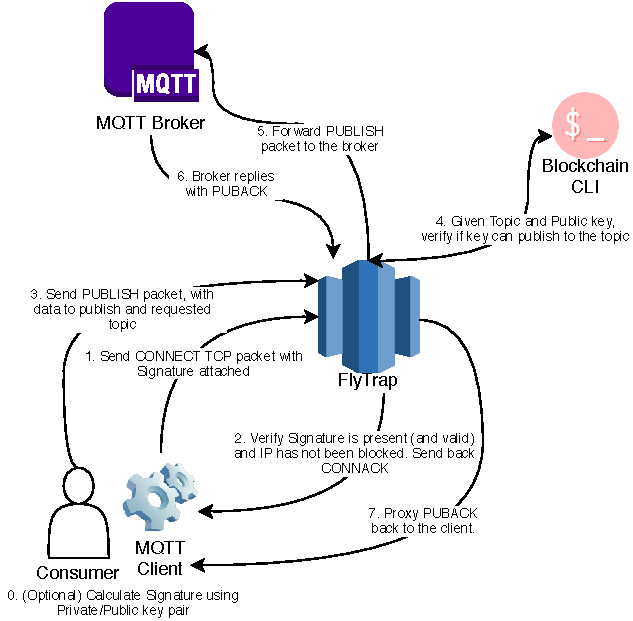
\includegraphics[width=0.8\textwidth]{workflow_success}
    \caption{Example successful workflow to publish a message on the broker through FlyTrap}
    \label{fig:workflow_success}
\end{figure}

Explanation of each step:
\begin{enumerate}\addtocounter{enumi}{-1}
    \item Marked as optional, since each Client can accept pre-computed signature, which can be loaded onto the device; this can be helpful for situations where there is not enough computational power for calculations. (\textbf{CL})
    \item Client sends CONNECT packet, including signature + public key in the optional fields of MQTT message. (\textbf{CL})
    \item FlyTrap will extract the signature from the optional field and then verify its integrity. It will also check if the client has not been attempting many unsuccessful connections. Finally, FlyTrap will repond with CONNACK, signaling to the client that it may now submit relevant payload packets. If the integrity check has failed, CONNACK would also have a flipped flag indicating rejected connection and cease further communication. (\textbf{CL})
    \item Client will now forward the relevant PUBLISH/SUBSCRIBE packet to FlyTrap (as it still believes that it's a regular MQTT broker). (\textbf{CL})
    \item FlyTrap will now extract requeste topic from the MQTT packet and communicate with the Blockchain, presenting Public Key and requested topic to verify whether data can be accessed. For this example, the access check was successful. (\textbf{BL})
    \item FlyTrap proxies (unchanged) PUBLISH packet to the actual MQTT broker. (\textbf{ML})
    \item MQTT broker will now respond with PUBACK, indicating successful PUBLISH. (\textbf{ML})
    \item Finally, FlyTrap will proxy the same PUBACK packet back to the initial client to let them know that the operation was successful - and at the end, gracefully terminate the connection. (\textbf{CL})
\end{enumerate}

\subsection{Sample failed PUBLISH workflow}
Operation similar as in the previous section with the difference being that this time connection is not allowed, as the presented Public Key is not allowed to publish information on the given topic. For the brevity sake, I will skip explaining steps 0-3 - as they are identical as with the successful scenario. I will also use the same notation to signify which layer is responsible for this operation.

\begin{enumerate}\addtocounter{enumi}{4}
    \item Having verified authenticity of Public Key, FlyTrap again tries to verify with the Smart Contract whether the client can access the topic. This time though, the reponse is negative and the client is not allowed to publish on the requested topic.
    \item FlyTrap will send PUBACK back to the client, setting reason code\footnote{https://docs.oasis-open.org/mqtt/mqtt/v5.0/os/mqtt-v5.0-os.html\#\_Toc3901124} to "Not authorized", at the same time terminating the connection with the client. To client, the situation is identical as with providing invalid username/password for a vanilla MQTT broker.
    \item Framework will verify with the cached values to check if the originating IP has not exceeded maximum number of allowed tries. If it did, it can place it on a blacklist and every subsequent connection will be denied for the specified time. In this example, that's 5 minutes. This step is optional
    \item If the ban happens, FlyTrap will also register a new transaction on the blockchain to persistently log this event for the purposes of checking potential attack spikes or generating reports w.r.t.  captured data. This step is also optional, as it depends on the previous one.
\end{enumerate}

Note: as you can see, the MQTT Broker is never connected to nor contacted with the potentially malicious message. FlyTrap rejects the message and forbids the connection. 
\begin{figure}[h]
    \centering
    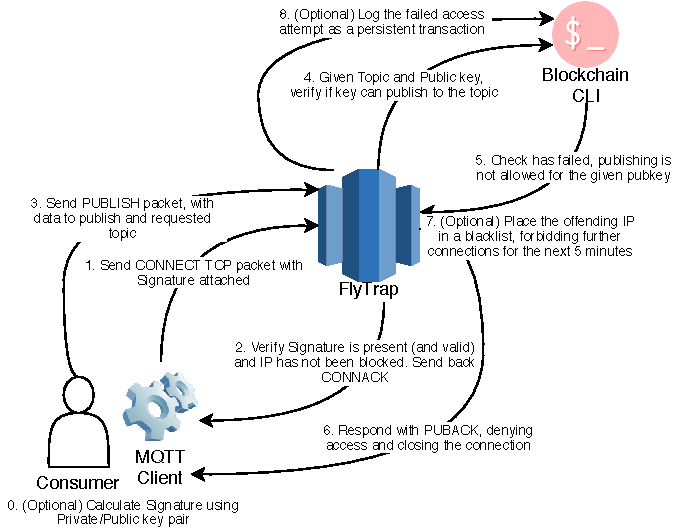
\includegraphics[width=0.9\textwidth]{workflow_fail}
    \caption{Example failed workflow to publish a message on the broker through FlyTrap}
    \label{fig:workflow_fail}
\end{figure}

\section{Consumer Layer}
First and foremost, the consumer layer. This part of the framework handles all connections between clients attempting to PUBLISH or SUBSCRIBE to data. To them, FlyTrap should be indistinguishable from a vanilla MQTT broker, which should be accepting all regular MQTT payloads. Though since every MQTT client produced in this project can connect with every MQTT Broker, a specific client is required for connection with FlyTrap - which is further explained in the section below. Moreover, an approach of identifing whether the client holds a Private Key for the presented Public Key is also needed and explained. 
\subsection{MQTT Client}
As mentioned above, FlyTrap makes use of the introduced in MQTT v5.0 User Properties\footnote{https://docs.oasis-open.org/mqtt/mqtt/v5.0/os/mqtt-v5.0-os.html\#\_Toc3901068}, allowing clients to include key-value pairs in the MQTT packets, which then can be utilised by the brokers (or other middleware). That's also where the signature and public key is being placed by the client when attempting connection with FlyTrap - and that's also the need for a custom client, since normal clients are not capable of producing highly specilised signatures for the purposes of connecting with Ethereum blockchain.

It is important to point out, the client is only slightly altered to provide (and compute if needed) the signature from public/private key pair. It is not a crucial system of the framework, as any client capable of setting User Properties for MQTT message would be sufficient, though for the purposes of this dissertation, custom implementation has also been designed and included.
\subsection{Secure Proxy}
In order to enable FlyTrap to make decisions on whether the requests for publishing or subscribing should be accepted or denied, a secure proxy needs to be established between the clients and the MQTT Broker. As the communication between the broker and the consumers happens on Transport Layer, it is possible to insert a middleman who would be capable of inspecting the packets flowing through, dissecting it for relevant information and finally make a decision about their future journey - all without the client ever knowing that someone has intercepted the connection. 
\begin{figure}[h]
    \centering
    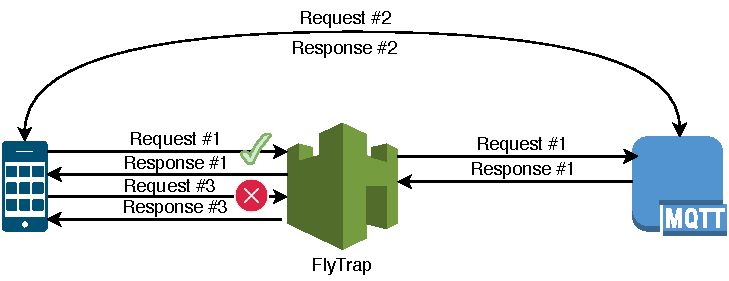
\includegraphics[width=0.8\textwidth]{tls}
    \caption{FlyTrap acting as a proxy}
    \label{fig:tls}
\end{figure}
Figure \ref{fig:tls} demonstrates all 3 possibilities when client attempts connection to a broker. In the Request \#1, FlyTrap will dissect the packet and confirm that the phone indeed can be allowed to access specific topic and then start bidirectional proxy with the broker, passing the TCP packets between two. Request \#2 shows that the same packet can be used for vanilla MQTT Broker without FlyTrap, thus decoupling the client and secure proxy, as the former can be used without the need to change the latter. Finally, for the third request, it is found that the client cannot access the requested resource and will be presented with CONACK response, with access denied flag set, terminating the connection. Though, in order to make such decisions, the proxy needs to inspect the contents of the packets.

Although this solution enough will not be sufficient, as quickly as FlyTrap can tap into the connection, the same can be assumed for potential malicious actors, which could be listening on the flowing through packets. The solution will support an extension to standard TCP - Transport Layer Security, or TLS for short, responsible for encrypting the TCP packets, significantly reducing the threat of man-in-the-middle attacks.

TLS sessions can be summarised in the following steps:
\begin{enumerate}
\item Initiate standard TCP session
\item ClientHello with client's cypher capabilities 
\item ServerHello and exchange of the cypher suite, along with server's certificate
\item Key exchange and change of cypher spec
\item Encrypted session starts
\end{enumerate}

It's important to point out, that due to step 3 requiring server's certificate, FlyTrap will need to either obtain a copy of broker's certificates or generate a new pair, ensuring that the connecting clients will trust it. Though, secure TLS connection remains optional, as it is understandable that sometimes enhanced security might cause undesirable performance losses or the MQTT broker simply doesn't support TLS connections - TLS will be configurable via command line arguments.

For every new connection, a new thread (or, go routine) is spawned which has its own context and is separated from others.

\subsection{Authenticity of public keys}
Public Keys from the Ethereum wallet are used as an identifier when determining whether client can access given resource or not. Though it only handles a part of the problem. Public Keys, by definition, are public, meaning that anyone could impersonate legitimate holders of the public/private key. This calls for an approach similar to the Certificate Authority problem when attempting encrypted HTTPS connections. Unfortunately, FlyTrap cannot expect every IoT device to have its own set of certificates, which would then need to be trusted by the framework in order to become recognisable - as those devices are often of limited storage and power.

To solve the problem of establishing whether the person presenting a public key also holds a corresponding key, signatures are used. Below you can see two figures, each outlining client side and FlyTrap side of the signing/verification process.

\begin{figure}[h]
    \centering
    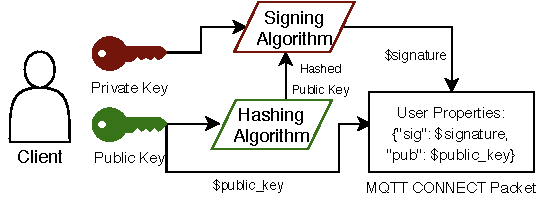
\includegraphics[width=0.8\textwidth]{sign}
    \caption{Client signing Public Key and attaching it to the message}
    \label{fig:sign}
\end{figure}

Figure \ref{fig:sign} shows how client - in possession of public/private key pair produces a signature which then is attached to the final MQTT CONNECT packet. First, it hashes the public key using Keccak-256 algorithm \cite{bertoni2009keccak} (commonly used in Ethereum, e.g. for block hashes), then it uses the private key to sign this hash and attaches obtained signature to the user properties part of the MQTT CONNECT message. Plain-text version of the public key is also attached in another field. Ethereum signatures are created by signing arbirtary bytes through generated private key - which then can only be verified using the corresponding public key. It is also possible to extract signed bytes from the same signature in the process.

\begin{figure}[h]
    \centering
     \makebox[\textwidth][c]{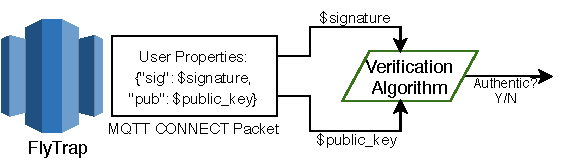
\includegraphics[width=1.1\textwidth]{verify}}
    \caption{FlyTrap verifying the signature}
    \label{fig:verify}
\end{figure}

Then, as per figure \ref{fig:verify}, FlyTrap receives the CONNECT packet and extracts both the signature \& public key from the message. As the corresponding private key for the public key was used to produce the signature, framework verifies this through Verification Algorithm. The output is a binary yes/no value - determining whether the public key was used to create the signature - along with the signed value (in this case, hashed public key) by the client. Then, framework can verify whether both signature was indeed created with the private key corresponding to the attached public key and (by hashing it again) compare the extracted value with the attached public key. This gives a definite answer that the person presenting the public key also holds the private key and thus is successfully authenticated.

For Ethereum, both Verification Algorithm and Signing Algorithm is part of Elliptic Curve Digital Signature Algorithm \citep{johnson2001elliptic}, where public key has exactly 160 bits (which, coincidentally, is also used for ETH addresses). Hashing Algorithm - as mentioned above - is Keccak-256.
\subsection{Protecting from brute-force attacks}
Some of the failed attempts can result in persistent log to blockchain, which often implicates costs - especially if FlyTrap is operating on a public blockchain. This can open a door for malicious actors attempting to drain the framework from available funds by logging a lot of operations in a short span of time. Distributed Denial of Service (DDoS) attacks can also occur and overload the server, which - depending on hardware - could only handle a limited number of simultaneous connections.

To combat those problems, framework will track any failed authentication attempts in an internal dictionary, mapping IP address to the number of failed attempts. This dictionary then will be consulted whenever a new connection is initiated. If it is, then the TCP link will be shut down and client informed that it is currently blacklisted. Though to give benefit of a doubt, there is a grace period of 2 prior failed attempts before a timed ban is applied. Whenever failed authentication occurs, the counter is increased by one - and if that count increases 3, the connection is terminated and dictionary updated with time 5 minutes in the future - that's the earliest time given IP can attempt connection again.
\section{Broker Layer}

This layer is where the communication with the actual MQTT Broker occurs. Normally, it would be desirable to place both FlyTrap and the broker (e.g. Mosquitto) on the same machine or at least network to minimise the latency - though it's not necessary. Depending on the outcome of the authorisation from the Client Layer, every packet from the client is forwarded to the broker and every packet from the broker sent back to the client. Since each connection is an individual thread, it also maintains information such as originating (\& destination) address and port - and this information will persist as long as the original connection Client <> FlyTrap remains open - which will only be terminated if client times out, requests disconnection or for any reason authentication to FlyTrap fails.

Similar to the section discussing encrypted connection, FlyTrap is capable of either connecting with TLS-capable brokers or via plain TCP if desired (though keeping the security implication in mind, as everyone intercepting the connection would be able to read the payload).

\section{Blockchain Layer}
In this layer, communication with the Ethereum Node occurs. As described in architecture section, FlyTrap can either read or write new data onto the chain. FlyTrap should be allocated its own smart contract containing chain code capable of verifying connecting clients and relevant data structures. Once that's done, 
\subsection{Data model}
The root of all communication with blockchain is a smart contract that contains all chaincode responsible for retrieving and storing information required by FlyTrap. Each organisation or entity willing to use FlyTrap should configure and deploy a new contract, which would be tied to a singular owner (i.e., a private key). Ethereum's chaincode execution can be limited to only particular set of addresses, here 
\begin{figure}[h]
    \centering
    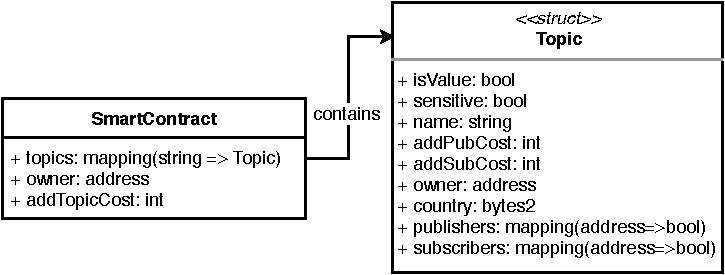
\includegraphics[width=0.9\textwidth]{uml_topic}
    \caption{Topic structure stored on Blockchain}
    \label{fig:uml_topic}
\end{figure}
\begin{figure}[h]
    \centering
    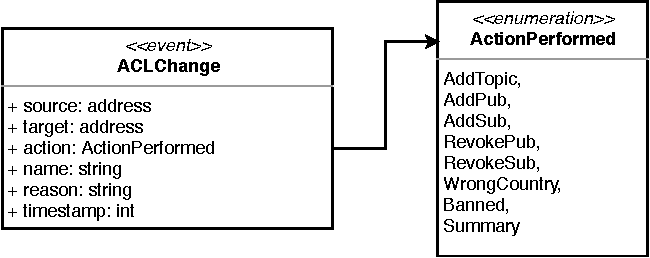
\includegraphics[width=0.9\textwidth]{uml_event}
    \caption{Event structure as stored in transaction log}
    \label{fig:uml_event}
\end{figure}
\subsection{Report Generation}
\subsection{Interacting with blockchain}
\section{Presentation Layer}
\subsection{Website}